\documentclass[12pt letter]{report}
\input{./template/preamble}
\input{./template/macros}
\input{./template/letterfonts}

\title{\Huge{Graphs}}
\author{\huge{Madiba Hudson-Quansah}}
\date{}
\usepackage{parskip}
\usepackage{tikz}
\usepackage{float}

\setcounter{tocdepth}{4}
\setcounter{secnumdepth}{4}

\begin{document}
\maketitle
\newpage
\pdfbookmark[section]{\contentsname}{too}
\tableofcontents
\pagebreak

\chapter{Graphs and Graph Models}

\section{Introduction}

\dfn{Graph}{
  A graph $G = \left( V, E \right) $ consist of $V$, a non empty set of \textit{vertices / nodes} and $E$ a set of
  \textit{edges}. Each edge has either one or two vertices associated with it called its \textit{endpoints}. An edge
  is said to \textit{connect} its endpoints. \\

  The set of vertices $V$ of a graph may be infinite, in this case the graph is called an \textit{infinite graph},
  conversely if the set of vertices is finite, the graph is called a \textit{finite graph}. \\

  The set of edges $E$ contains ordered pairs or sets of elements in the set of vertices $V$ indicating a connection between the
  two nodes or a node to itself.
}

\dfn{Vertex}{
  A \textit{vertex} is a point in a graph. \\
}

\dfn{Edge}{
  An \textit{edge} is a line connecting two vertices in a graph.
}

Below is a graph representing a network of data centres and communication links between computers, where locations are
represented by points and the links are represented by lines connecting the points.

\begin{figure}[H]
  \begin{center}
    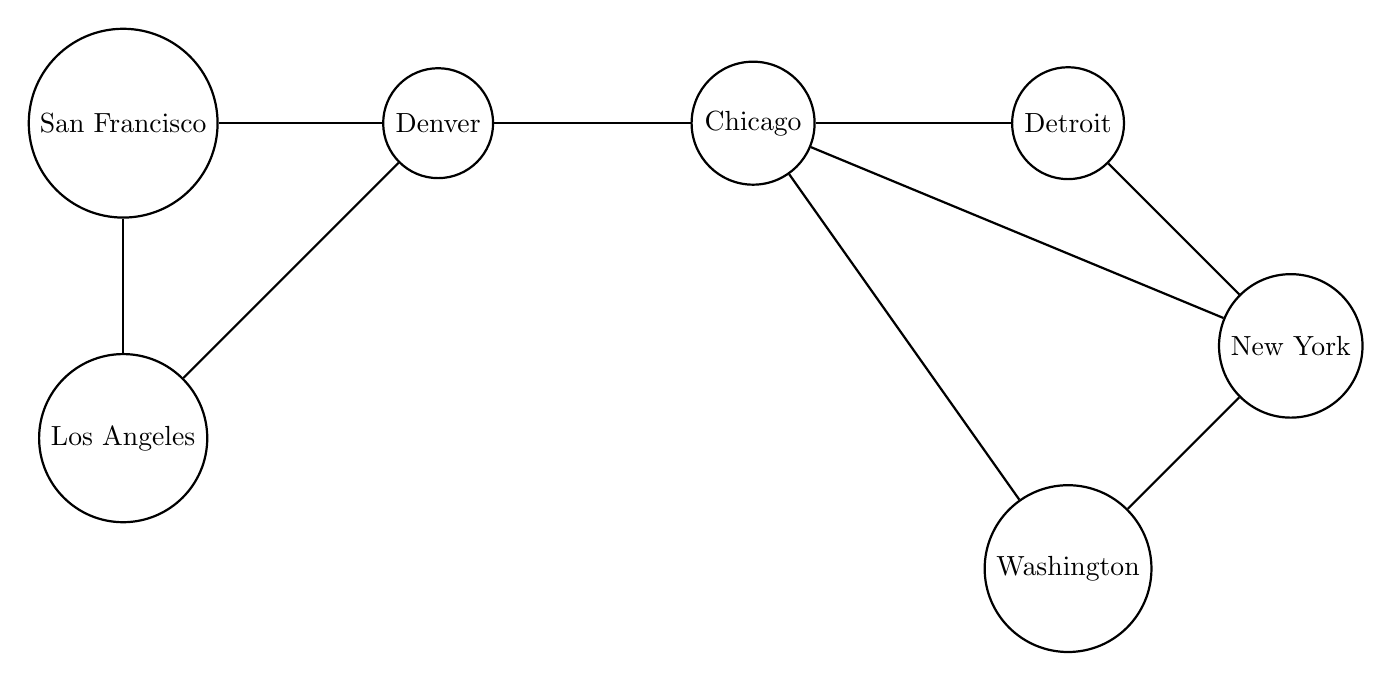
\begin{tikzpicture}[node distance={4cm}, thick, scale=0.5, main/.style = {draw, circle}]
      \node[main] (1) {San Francisco};
      \node[main] (2) [below of=1] {Los Angeles};
      \draw (1) -- (2);
      \node[main] (3) [right of=1] {Denver};
      \draw (1) -- (3);
      \draw (2) -- (3);
      \node[main](4) [right of=3]{Chicago};
      \draw (3) -- (4);
      \node[main] (5) [right of=4] {Detroit};
      \node[main] (6) [below right of=5] {New York};
      \node[main] (7) [below left of=6] {Washington};
      \draw (4) -- (5);
      \draw (4) -- (6);
      \draw (4) -- (7);
      \draw (5) -- (6);
      \draw (6) -- (7);
    \end{tikzpicture}
  \end{center}
  \label{fig:ex1}
\end{figure}

This is an example of a simple graph.

\dfn{Simple Graph}{
  A graph is said to be \textit{simple} if it has no loops or multiple edges. A \textit{loop} is an edge that connects
  a vertex to itself. A \textit{multiple edge} is two or more edges that connect the same pair of vertices. \\
}

\subsection{Multigraph}
This graph could be re-drawn to model multiple links between the same pair of locations, as shown in Figure \ref{fig:ex2}.

\begin{figure}[H]
  \begin{center}
    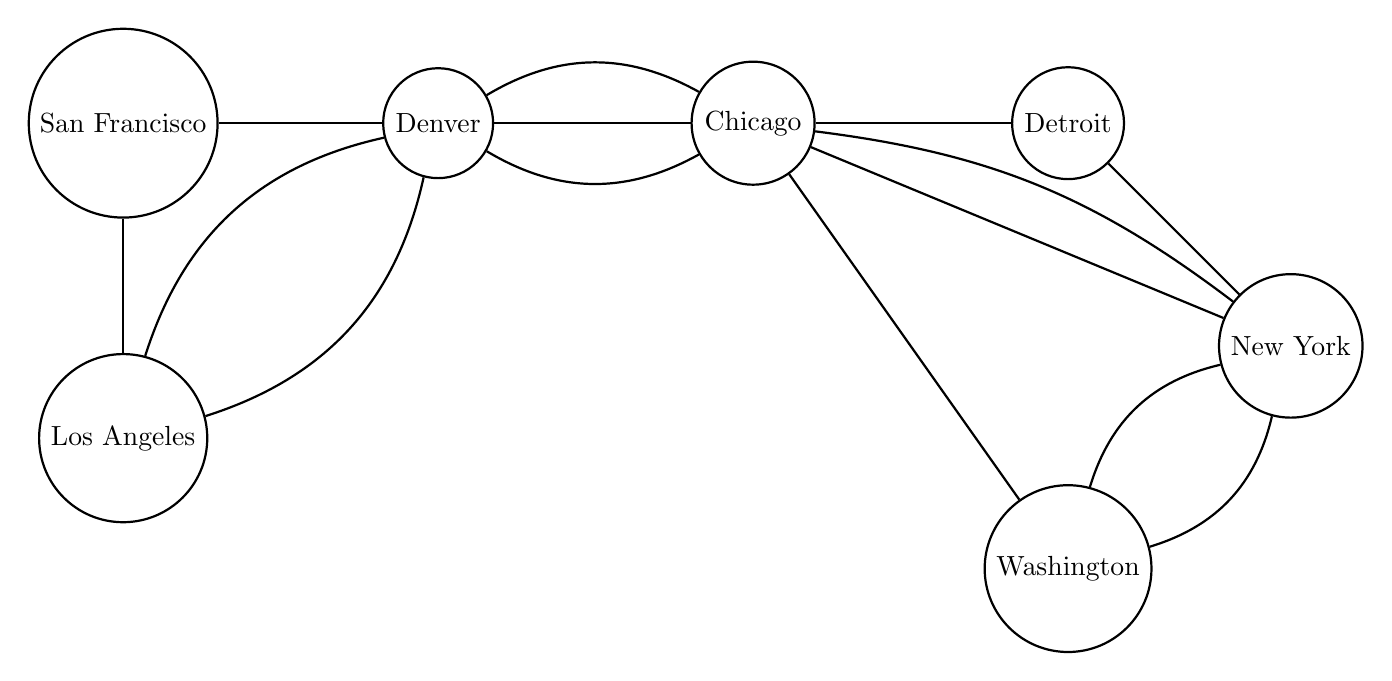
\begin{tikzpicture}[node distance={4cm}, thick, scale=0.5, main/.style = {draw, circle}]
      \node[main] (1) {San Francisco};
      \node[main] (2) [below of=1] {Los Angeles};
      \node[main] (3) [right of=1] {Denver};
      \node[main](4) [right of=3]{Chicago};
      \node[main] (5) [right of=4] {Detroit};
      \node[main] (6) [below right of=5] {New York};
      \node[main] (7) [below left of=6] {Washington};

      \path[every node/.style={font=\sffamily\small}]
      (1) edge (2)
      (1) edge (3)
      (2) edge [bend left] (3)
      (2) edge [bend right] (3)
      (3) edge (4)
      (3) edge [bend right] (4)
      (3) edge [bend left] (4)
      (4) edge (5)
      (4) edge [bend left=15] (6)
      (4) edge (6)
      (5) edge (6)
      (4) edge (7)
      (6) edge[bend right] (7)
      (6) edge[bend left] (7);
    \end{tikzpicture}
  \end{center}
  \label{fig:ex2}
\end{figure}
This is an example of a multigraph.

\dfn{Multigraph}{
  A graph that has multiple edges connecting the same vertices. When there are $m$ distinct edges connecting the same
  unordered pair of vertices $\{u, v\} $, we say that $\{u, v\} $ is an edge of \textit{multiplicity} $m$. i.e. j

}

\subsection{Loops}
Sometimes vertices may be connected to themselves, as shown in Figure \ref{fig:ex3}.
\begin{figure}[H]
  \begin{center}
    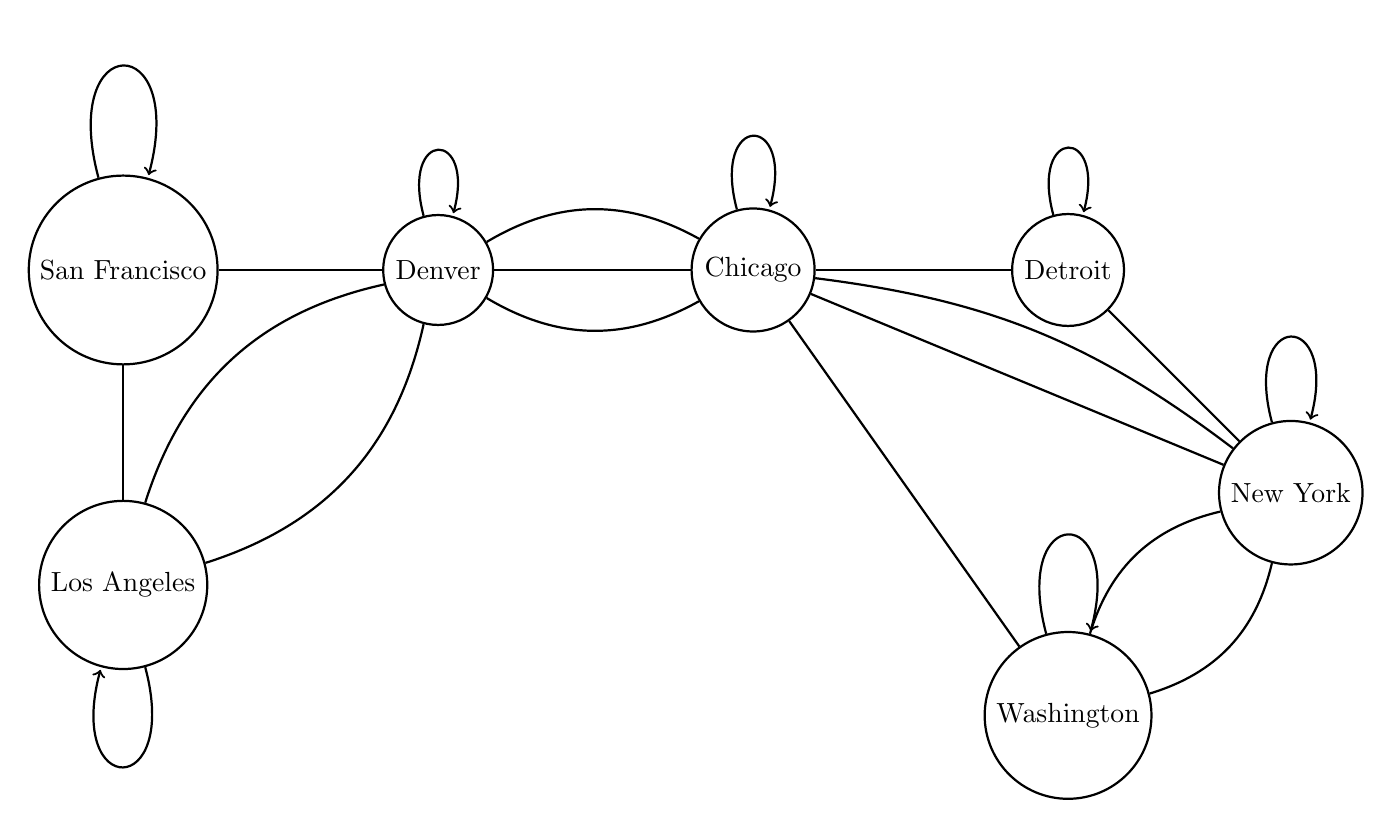
\begin{tikzpicture}[node distance={4cm}, thick, scale=0.5, main/.style = {draw, circle}]
      \node[main] (1) {San Francisco};
      \node[main] (2) [below of=1] {Los Angeles};
      \node[main] (3) [right of=1] {Denver};
      \node[main](4) [right of=3]{Chicago};
      \node[main] (5) [right of=4] {Detroit};
      \node[main] (6) [below right of=5] {New York};
      \node[main] (7) [below left of=6] {Washington};

      \path[every node/.style={font=\sffamily\small}]
      (1) edge [loop above] (1)
      (2) edge [loop below] (2)
      (3) edge [loop above] (3)
      (4) edge [loop above] (4)
      (5) edge [loop above] (5)
      (6) edge [loop above] (6)
      (7) edge [loop above] (7)
      (1) edge (2)
      (1) edge (3)
      (2) edge [bend left] (3)
      (2) edge [bend right] (3)
      (3) edge (4)
      (3) edge [bend right] (4)
      (3) edge [bend left] (4)
      (4) edge (5)
      (4) edge [bend left=15] (6)
      (4) edge (6)
      (5) edge (6)
      (4) edge (7)
      (6) edge[bend right] (7)
      (6) edge[bend left] (7);
    \end{tikzpicture}
  \end{center}
  \label{fig:ex3}
\end{figure}

Edges connecting vertices to themselves are called \textit{loops}.
\dfn{Loop}{
  An edge that connects a vertex to itself.
}

\dfn{Psuedograph}{
  A graph that allows loops and multiple edges.

}

\subsection{Directed Graphs}
So far the examples given have been \textit{undirected graphs}, with undirected edges. It is also possible to assign
directions to the edges, as shown in Figure \ref{fig:ex4}.

\begin{figure}[H]
  \begin{center}
    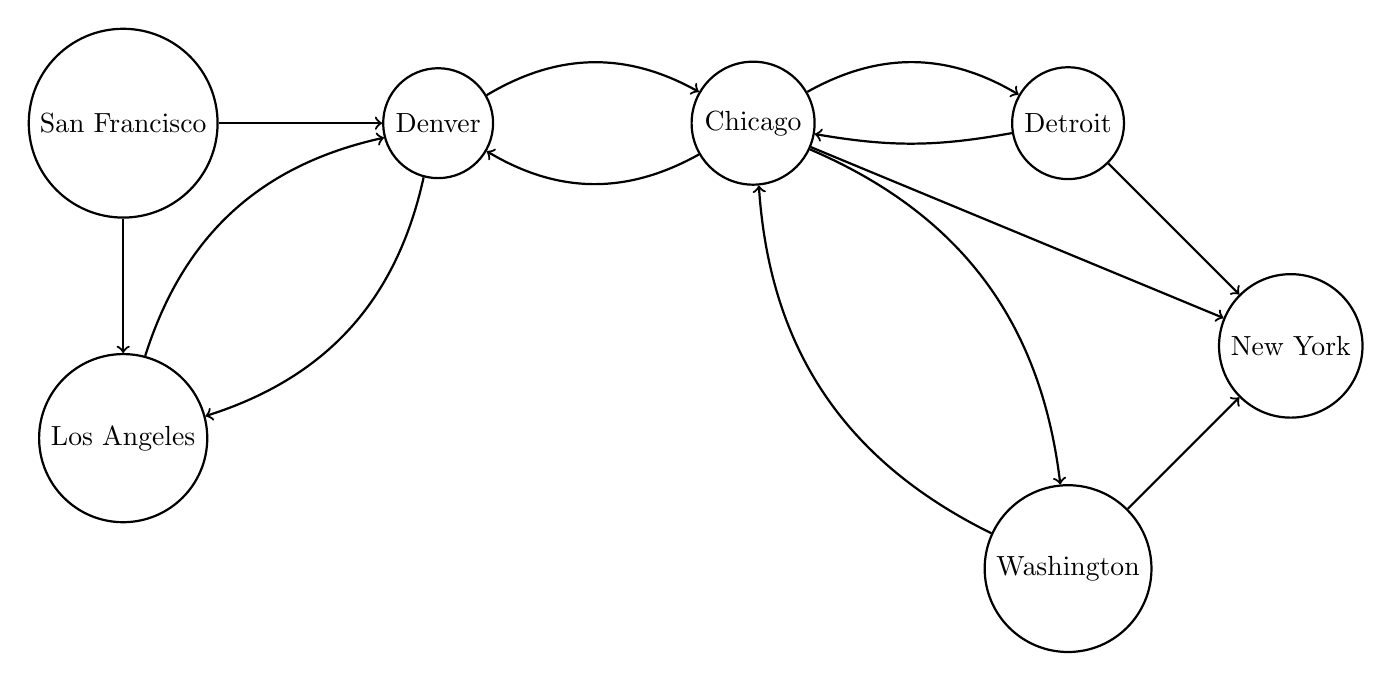
\begin{tikzpicture}[node distance={4cm}, thick, main/.style = {draw, circle}]
      \node[main] (1) {San Francisco};
      \node[main] (2) [below of=1] {Los Angeles};
      \node[main] (3) [right of=1] {Denver};
      \node[main](4) [right of=3]{Chicago};
      \node[main] (5) [right of=4] {Detroit};
      \node[main] (6) [below right of=5] {New York};
      \node[main] (7) [below left of=6] {Washington};

      \path[every node/.style={font=\sffamily\small}]
      (1) edge[->] (2)
      (1) edge[->] (3)
      (2) edge [bend left, ->] (3)
      (2) edge [bend right, <-] (3)
      (3) edge [bend right, <-] (4)
      (3) edge [bend left, ->] (4)
      (4) edge[bend left, ->] (5)
      (4) edge[bend right=10, <-] (5)
      (4) edge[->] (6)
      (5) edge[->] (6)
      (4) edge[bend left, ->] (7)
      (4) edge[bend right, <-] (7)
      (6) edge[<-] (7);
    \end{tikzpicture}
  \end{center}
  \label{fig:ex4}
\end{figure}

Such a graph is called a \textit{directed graph} or \textit{digraph}.

\dfn{Directed Graph}{
  A graph $\left( V, E \right) $ that consists of a non-empty set of vertices $V$ and a set of directed edges / arcs
  $E$. Each directed edge is associated with an ordered pair of vertices. The arc associated with the ordered pair
  $\left( u, v \right) $ is said to \textit{start} at $u$ and \textit{end} at $v$.
}

\subsection{Simple Directed Graph}
\dfn{Simple Directed Graph}{
  A directed graph with no loops or multiple edges.
}

\subsection{Directed Multigraph}
\dfn{Directed Multigraph}{
  A directed graph with multiple edges connecting the same pair of vertices. When there are $m$ directed edges, each
  associated to an ordered pair of vertices $\left( u, v \right) $, then $\left( u, v \right) $ is an edge of
  multiplicity $m$.
}

\subsection{Mixed Graph}
\dfn{Mixed graph}{
  A graph with both direct and undirected edges, that may have multiple edges and loops.
}

\subsection{Graph Terminology}

\begin{table}[htpb]
  \centering
  \begin{tabular}{|c|c|c|c|}
    \hline
    \textit{Type}         & \textit{Edges}          & \textit{Multiple Edges Allowed?} & \textit{Loops Allowed?} \\ [0.5ex]
    \hline
    \hline
    Simple graph          & Undirected              & No                               & No                      \\
    Multigraph            & Undirected              & Yes                              & No                      \\
    Psuedograph           & Undirected              & Yes                              & Yes                     \\
    Simple Directed Graph & Directed                & No                               & No                      \\
    Directed Multigraph   & Directed                & Yes                              & Yes                     \\
    Mixed Graph           & Directed and Undirected & Yes                              & Yes                     \\
    \hline
  \end{tabular}
  \caption{Graph Terminology}
  \label{tab:grp1}
\end{table}

\chapter{Graph Terminology and Special Graphs}

\section{Basic Terminology}

\dfn{Adjacent / Neighbours }{
  Two vertices $u$ and $v$ in an undirected graph $G$, that are endpoints of an edge $e$. Such an edge $e$ is called
  \textit{incident with} the nodes $u$ and $v$ and $e$ is said to \textit{connect} $u$ and $u$
}

\dfn{Neighbourhood}{
  The set of all neighbours of a vertex $v$ of $G = \left( V, E \right) $, denoted by:
  \[
    N \left( v \right)
  \]
  If $A$ is a subset of $V$, we denote by $N \left( A \right) $ the set of all nodes in $G$ that are adjacent to at least one node
  in $A$. i.e. $N \left( A \right) = \bigcup_{v \in A} N \left( v \right)$
}

\dfn{Degree of a Vertex / Node}{
  The number of edges incident with a particular node, except that a loop at a node is counted twice to the degree of
  that node, denoted by:
  \[
    \text{deg}\left( v \right)
  \]
}

\ex{}{
  \qs{}{
    What are the degrees and neighbourhoods of the vertices of the graph below \\

    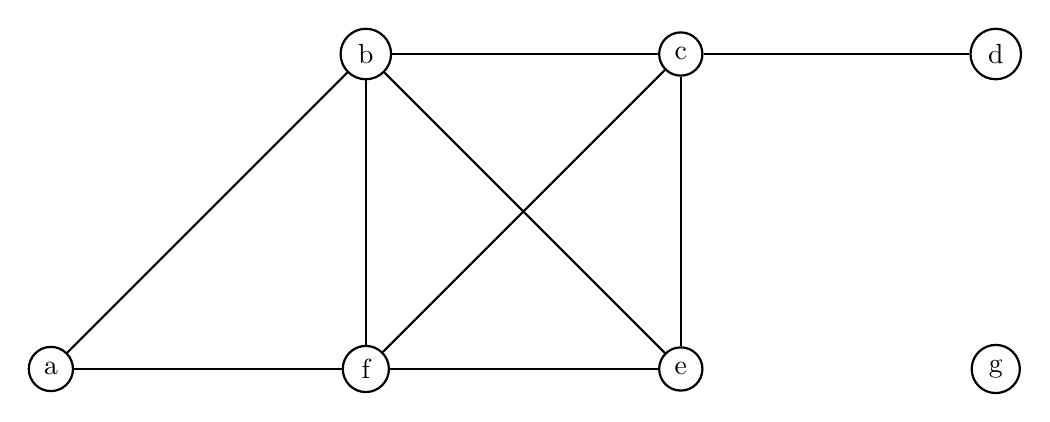
\begin{tikzpicture}[node distance={4cm}, thick, scale=0.5, main/.style = {draw, circle}]
      \node[main] (1) {a};
      \node[main] (2) [right of=1] {f};
      \node[main] (3)[above of=2]{b};
      \node[main](4)[right of=3]{c};
      \node[main](5)[right of=2]{e};
      \node[main](6)[right of=4]{d};
      \node[main](7)[right of=5]{g};
      \path
      (1) edge (2)
      (1) edge (3)
      (3) edge (4)
      (3) edge (5)
      (3) edge (2)
      (2) edge (4)
      (4) edge (5)
      (5) edge (2)
      (4) edge (6)
      ;
    \end{tikzpicture}
  }

  \sol{

    \noindent \underline{Degrees:} \\
    \\
    deg(a) - $2$\\
    deg(b) - $4$\\
    deg(c) - $4$ \\
    deg(d) - $1$\\
    deg(e) - $3$ \\
    deg(f) - $4$ \\
    deg(g) - $0$ \\

    \noindent \underline{Neighbourhoods:}\\
    \\
    \begin{align*}
      N \left( a \right) & = \{b, f\}       \\
      N \left( b \right) & = \{c, f, e, a\} \\
      N \left( c\right)  & = \{b, d, f, e\} \\
      N \left( d \right) & = \{c\}          \\
      N \left( e \right) & = \{b, f, c\}    \\
      N \left( f \right) & = \{b, c, e, a\} \\
      N \left( g \right) & = \O
    \end{align*}
  }
}

\thm{The Handshaking Theorem}{
  Let $G = \left( V, E \right) $ be an undirected graph with $m$ edges. Then
  \[
    2m = \displaystyle\sum_{v \in V} \text{deg}\left( v \right)
  \]
}

\thm{}{
  An undirected graph has an even number of nodes of odd degree.
}


\end{document}
